\begin{title}
  Интегрирование ФМП
\end{title}

\begin{title}[\Large]
  Определение кратного интеграла. Критерий интегрируемости
\end{title}

\begin{block}[Обозначения]
  $f(x)$ определена и измерена по Жорадану множества $E \subset R^n$

  $R(E) = \{E_k\}$ разбиение

  $E = \sqcup_{k=1}^L E_k$

  $d(E_k) = \sup \limits_{x,y \in E_k} \rho(x,y)$ диаметр множества $E_k$

  $\lambda(R) = \max \limits_{1 \le k \le L} d(E_k)$ мелкость разбиения

  $m_k = \inf \limits_{x \in E_k} f(x) ~~~ M_k = \sup \limits_{x \in E_k} f(x)$

  $\sum_{k=1}^L f(x^{(k)}) m(E_k)$ называется итегральной суммой для $f$
  соответствующее разбиению $R(E)$ и выборки $\upsilon(R) = \{x^{(k)}\} ~~
  x^{(k)} \in E_k$

  $\sum_{k=1}^L m_k m(E_k) = \int_* (R)$ нижняя сумма Дарбу

  $\sum_{k=1}^L M_k m(E_k) = \int^* (R)$ верхняя сумма Дарбу
\end{block}

\begin{define}[кратного интеграла]
  $$
  \forall \varepsilon > 0 ~~~ \exists \delta_{\varepsilon} > 0 ~~~
  \forall R(E) ~~~ \lambda(R) < \delta_{\varepsilon} ~~~
  \forall \upsilon(R) ~~~ \left| \sum_{k=1}^L f(x^{(k)}) m(E_k) - I \right|
  < \varepsilon
  $$
  число $I$ называется кратным интегралом и обозначают
  $$
  \int_E f(x) dx = \int_E f(x) dm
  $$
  $$
  \iint_E f(x,y) dxdy ~~ \text{двойной интеграл}
  $$
  $$
  \iiint_E f(x,y,z) dxdydz ~~ \text{тройной интеграл}
  $$
  Если кратный интеграл функции на множестве $E$ существует то $f(x)$
  называется интегрируемой по мере Жорадана.

  Если $n \ge 2$ то ограничение не является необходимым условием
  интегрирования функции.
\end{define}

\begin{block}[Критерий интегрируемости кратного интеграла]
  Для того чтобы $f(x)$ была интегрируема на измеренным по Жордану множестве
  $E \subset R^n$ необходимо и достаточно

  1) ограничена

  2)
  $$
  \forall \varepsilon > 0 ~~~ \exists \delta_{\varepsilon} > 0 ~~~ \forall R(E)
  ~~~ \lambda(R) < \delta_{\varepsilon} ~~~ \left| \int^*(R) - \int_*(R)
  \right| < \varepsilon
  $$
\end{block}

\begin{title}[\Large]
  Классы интегрируемых ФМП. Мера цилиндричского тела. Мера Жордана графика
  интегрируемой функции
\end{title}

\begin{theorem}
  $f(x)$ непрерывна на компактном множестве $E$ измеренным по Жордану тогда
  $f(x)$ интегрируема на $E$.
\end{theorem}

\begin{proof}
  $$
  \forall \varepsilon > 0 ~~~ \exists \delta_{\varepsilon} > 0 ~~~ \forall R
  ~~~  \lambda(R) \subset \delta_{\varepsilon} ~~~
  \left| \int^*(R) - \int_*(R) \right| < \varepsilon
  $$
  $$
  \forall \varepsilon > 0 ~~~ \exists \delta_{\varepsilon} > 0 ~~~
  x', x'' \in E ~~~ \rho (x', x'') \le \delta_{\varepsilon} ~~~
  |f(x') - f(x'')| < \varepsilon
  $$
  $$
  \int^*(R) - \int_*(R) \le \sum_{k=1}^m(M_k - m_k)m(E_k^*) =
  $$
  $$
  = \sum_{k=1}^m (f(x'^{(k)}) - f(x''^{(k)}))m(E_k^*) < \frac{\varepsilon}{m(E)}
  \sum_{k=1}^m m(E_k^*) = \frac{\varepsilon}{m(E)} m(E) = \varepsilon
  $$
\end{proof}

\begin{define}[Жораданова множетеля $0$]
  $$
  \forall \varepsilon > 0 ~~~ \exists B_{\varepsilon} ~~~ E \subset
  B_{\varepsilon} ~~~ m(B_{\varepsilon}) < \varepsilon
  $$
\end{define}

\begin{theorem}
  $f(x)$ ограничена на компактном множестве $E$ и непрерывна на $E$ за
  исключением меры Жорданова $m(E)=0$ тогда $f(x)$ интегрируема на $E$.
\end{theorem}

\begin{define}[цилиндра]
  $$
  E_h = \{ (x_1, x_2, \ldots, x_n, x_{n+1}): ~ (x_1, x_2, \ldots, x_n) \in E
  ~~ 0 \le x_{n+1} \le h\}
  $$
  цилиндр с основанием $E$ и высотой $h$
\end{define}

\begin{block}[Лемма]
  $E \subset R^n ~~~ m(E)$ измемерена тогда $m(E)h = m(E_h)$
\end{block}

\begin{proof}
  $$
  \forall \varepsilon > 0 ~~~ \exists A_{\varepsilon}, B_{\varepsilon} ~~~
  A_{\varepsilon} \subset E \subset B_{\varepsilon}
  ~~~ m(B_{\varepsilon}) - m(A_{\varepsilon}) < \frac{\varepsilon}{h}
  $$
  $$
  m(A_{\varepsilon h}) = hm(A_{\varepsilon}) ~~~ m(B_{\varepsilon h}) =
  hm(B_{\varepsilon})
  $$
  $$
  A_{\varepsilon h} \subset E_h \subset B_{\varepsilon h} ~~~
  m(B_{\varepsilon h}) - m(A_{\varepsilon h}) \le h(m(B_{\varepsilon}) -
  m(A_{\varepsilon})) < \varepsilon
  $$
  $$
  m(A_{\varepsilon h}) \le m(E_h) \le m(B_{\varepsilon h})
  $$
  $$
  hm(A_{\varepsilon}) \le hm(E) \le hm(B_{\varepsilon})
  $$
  $$
  m(A_{\varepsilon}) \le m(E) \le m(B_{\varepsilon})
  $$
  $$
  m(E_h) - hm(E) \le m(B_{\varepsilon h}) - m(A_{\varepsilon h}) < \varepsilon
  $$
\end{proof}

\begin{define}[графика функции]
  $$
  \Gr f = \{ (x_1, x_2, \ldots, x_n, x_{n+1}): ~ (x_1, x_2, \ldots, x_n) \in E
  ~~ x_{n+1} = f(x_1, x_2, \ldots, x_n) \}
  $$
\end{define}

\begin{theorem}
  $f(x)$ интегрируема на измеренным по Жордану множестве $E \subset R^n$ тогда
  ее $\Gr f$ с $m(E) = 0$ в $R^{n+1}$
\end{theorem}

\begin{proof}
  $m(E) > 0$ так как $E$ измерима по Жордану
  $$
  \forall \varepsilon > 0 ~~~ A_{\varepsilon} \subset E \subset B_{\varepsilon}
  ~~~ m(B_{\varepsilon}) - m(A_{\varepsilon}) < \frac{\varepsilon}{m(E)}
  $$
  пусть $R(E) = \{E_k\} ~~~ A_{\varepsilon} = \sqcup_{k=1}^n A_k ~~~
  B_{\varepsilon} = \sqcup_{k=1}^n B_k$
  $$
  \sqcup_{k=1}^n A_{k m_k} \subset \Gr f \subset \sqcup_{k=1}^n B_{k M_k}
  $$
  $$
  \Gr f \subset \sqcup_{k=1}^m (B_{k M_k} - A_{k m_k})
  $$
  $$
  m(\Gr f) \le \sum_{k=1}^m (M_k - m_k)m(E_k) =
  \int^* (R) - \int_* (R) < \varepsilon \Rightarrow
  $$
  $$
  m(\Gr f) = m(E) = 0
  $$
\end{proof}

\begin{block}[Следствие]
  График любой непрерывной $f$ на компактном множестве $E \subset R^n$ имеет
  $m(E)=0$ в $R^{n+1}$
\end{block}

\begin{title}[\Large]
  Свойства кратных интегралов
\end{title}

\begin{block}[Свойства]
  1) $\int_E 1 dx = m(E)$

  2) $\forall x \in E \subset R^n ~~~ f(x) > 0$ тогда $\int_E f(x) dx \ge 0$

  3) $\alpha, \beta \in R ~~~ f(x), g(x)$ интегрируемы на $E$ тогда
  $$
  \exists \int_E (\alpha f(x) + \beta g(x)) dx = \alpha \int_E f(x)dx +
  \beta \int_E g(x) dx
  $$
  4) $f(x), g(x)$ интегрируема на $E$ тогда $f \cdot g$ интегрируема

  5) $f(x)$ интегрируема на $E$ и $|f(x)|$ интегрируема на $E$ тогда
  $$
  \left| \int_E f(x) dx \right| \le \int_E |f(x)|dx
  $$
  6)
  $$
  E = \sqcup_{k=1}^m E_k ~~~ \int_E f(x) dx = \sum_{k=1}^m \int_{E_k} f(x) dx
  $$
\end{block}

\begin{theorem}[о среднем]
  $f(x)$ непрерывна на компактном и связанном множестве $E$ тогда
  $\exists c \in E$
  $$
  \int_E f(x)dx = f(c) m(E)
  $$
\end{theorem}

\begin{proof}
  $m(E) > 0$ так как $f$ непрерывна на $E$ тогда
  $$
  \exists \mu = \inf \limits_{x \in E} f(x) ~~~ \nu = \sup \limits_{x \in E}
  f(x) ~~~ \mu \le f(x) \le \nu
  $$
  $$
  \int_E \mu dx \le \int_E f(x) dx \le \int_E \nu dx
  $$
  $$
  \mu m(E) \le \int_E f(x) dx \le \nu m(E)
  $$
  $$
  \mu \le \frac{\int_E f(x)dx}{m(E)} \le \nu
  $$
  по Коши
  $$
  \exists c \in E ~~~ f(c) = \frac{\int_E f(x)dx}{m(E)}
  $$
\end{proof}

\begin{title}[\Large]
  Сведение двойного интеграла по прямоугольнику к повторному интегралу
\end{title}

\begin{theorem}
  1) $f(x, y)$ ограничена на прямоугольнике $[a,b] \times [c,d] = \Pi$

  2) $\exists \iint_{\Pi} (x,y)dxdy$

  3) $\forall x \in [a,b] ~~~ \exists \int_c^d f(x,y) dy = F(x)$

  тогда

  1) $F(x)$ интегрируема на $[a,b]$

  2)
  $$
  \iint_{\Pi} f(x, y) dxdy = \int_a^b F(x)dx = \int_a^b \left( \int_c^d f(x,y)
  dy \right)dx = \int_a^b dx \int_c^d f(x,y) dy
  $$
  повторный интеграл

  Замечание: если 3 условие заменить на
  $\forall y \in [c,d] ~~~ \exists \int_a^b f(x,y) dx = \Phi(y)$
  $$
  \iint_{\Pi} f(x, y) dxdy = \int_c^d \Phi(y)dy = \int_c^d dy \int_a^b f(x,y) dx
  $$
\end{theorem}

\begin{proof}
  $R_1([a,b]) = \{x_i\} ~~~ i = 1,2, \ldots, n$

  $R_2([c,d]) = \{y_i\} ~~~ j = 1,2, \ldots, m$

  $\Delta_{ij} = [x_{i-1}, x_i] \times [y_{j-1}, y_j] ~~~ \Pi =
  \sqcup_{i=1}^n \sqcup_{j=1}^m \Delta_{ij}$

  $$
  M_{ij} = \sup_{(x,y) \in \Delta_{ij}} f(x,y) ~~~
  m_{ij} = \inf_{(x,y) \in \Delta_{ij}} f(x,y) ~~~ y_{\Delta j} = y_j - y_{j-1}
  ~~~ x_{\Delta i} = x_i - x_{i-1}
  $$
  $$
  m_{ij} y_{\Delta i} \le \int_{y_i-1}^{y_i} f(x,y)dy \le M_{ij} y_{\Delta j}
  ~~~ j = 1, 2, \ldots, m
  $$
  $$
  \sum_{j=1}^m m_{ij} y_{\Delta i} \le \sum_{j=1}^m \int_{y_i-1}^{y_i} f(x,y)dy
  \le \sum_{j=1}^m M_{ij} y_{\Delta j}
  $$
  $$
  \sum_{j=1}^m m_{ij} y_{\Delta i} \le \int_c^d f(x,y)dy \le \sum_{j=1}^m
  M_{ij} y_{\Delta j}
  $$
  $$
  M_i = \sup_{x \in [x_{i-1}, x_i]} F(x) ~~~ m_i =
  \inf_{x \in [x_{i-1}, x_i]} F(x)
  $$
  $$
  \sum_{j=1}^m m_{ij} y_{\Delta i} \le m_i \le M_i \le \sum_{j=1}^m
  M_{ij} y_{\Delta j}
  $$
  $$
  0 \le M_i - m_i \le \sum_{j=1}^m (M_{ij} - m_{ij}) y_{\Delta j}
  $$
  $$
  0 \le \sum_{i=1}^n (M_i - m_i)x_{\Delta i} \le \sum_{i=1}^n \sum_{j=1}^m
  (M_{ij} - m_{ij}) y_{\Delta j} x_{\Delta i}
  $$
  $R(\Pi) = R_1([a,b]) \times R_2([c,d]) = \{ \Delta_{ij} \}$
  $$
  \int^*(R_1) - \int_*(R_1) \le \int^*(R) - \int_*(R)
  $$
  так как по условию 2 $f(x,y)$ интегририрема по прямоугольнику $\Pi$ тогда
  если $\lambda(R_1) < \lambda(R) < \delta_{\varepsilon}$
  $$
  \int^*(R_1) - \int_*(R_1) \le \int^*(R) - \int_*(R) < \varepsilon
  $$
  по критерию интегрируемости $F(x)$ интегрируема на $[a,b]$

  вернемся к
  $$
  \sum_{j=1}^m m_{ij} y_{\Delta i} \le \int_c^d f(x,y)dy \le \sum_{j=1}^m
  M_{ij} y_{\Delta j}
  $$
  $$
  \sum_{j=1}^m m_{ij} y_{\Delta i} \le \int_{x_i-1}^{x_i} \int_c^d f(x,y)dy \le
  \sum_{j=1}^m M_{ij} y_{\Delta j}
  $$
  $$
  \sum_{i=1}^n \sum_{j=1}^m m_{ij} y_{\Delta i} \le \sum_{i=1}^n
  \int_{x_i-1}^{x_i} dx \int_c^d f(x,y)dy \le \sum_{i=1}^n \sum_{j=1}^m
  M_{ij} y_{\Delta j}
  $$
  $$
  \sum_{i=1}^n \sum_{j=1}^m m_{ij} y_{\Delta i} \le \int_a^b dx
  \int_c^d f(x,y)dy \le \sum_{i=1}^n \sum_{j=1}^m M_{ij} y_{\Delta j}
  $$
  $$
  \int_*(R) \le \int_a^b dx \int_c^d f(x,y)dy \le \int^*(R)
  $$
  $$
  \int_*(R) \le \iint_{\Pi} f(x,y)dx dy \le \int^*(R)
  $$
  $$
  \left| \iint_{\Pi} f(x,y)dx dy - \int_a^b dx \int_c^d f(x,y)dy \right| \le
  \int^*(R) - \int_*(R) < \varepsilon
  $$
\end{proof}

\begin{block}[Следствие]
  $f(x,y)$ непрерывна в прямоугольнике $[a,b] \times [c,d]$ тогда
  $$
  \iint_{\Pi} f(x,y) dxdy = \int_a^b dx \int_c^d f(x,y) dy =
  \int_c^d dy \int_a^b f(x,y) dx
  $$
\end{block}

\begin{title}[\Large]
  Сведение двойного интеграла к повторному в случа области произвольного вида
\end{title}

\begin{theorem}
  $f(x,y)$ определена и непрерывна на $E = \{ (x,y) : a < x < b ~~
  \varphi(x) \le y \le \psi(x) \}$ где $\varphi(x), \phi(x)$ непрерывны на
  $[a,b]$ тогда
  $$
  \iint_E f(x,y)dxdy = \int_a^b dx \int_{\varphi(x)}^{\phi(x)} f(x,y)dy
  $$
\end{theorem}

\begin{proof}
  $0 \le \varphi(x) \le y \le \phi(x)$

  $\Pi = [a,b] \times [c,d]$
  $$
  F(x,y) =
  \left\{
  \begin{array}{cc}
    f(x,y) &(x,y) \in E \\
    0 & (x,y) \in \Pi \backslash E
  \end{array}
  \right.
  $$
  множество точек имеет разрыв $m(E) = 0$ $\Rightarrow$ $F(x,y)$ интегрируема
  на $\Pi$
  $$
  \iint_{\Pi} F(x,y) dxdy = \int_a^b dx \int_c^d F(x,y) dy =
  $$
  $$
  = \iint_{\Pi \backslash E} F(x,y) dxdy + \iint_E F(x,y)dxdy =
  $$
  $$
  = \int_a^b dx \left( \int_a^{\varphi(x)} F(x, y) dy +
  \int_{\varphi(x)}^{\phi(x)} F(x, y) dy \right)
  $$
  $$
  \iint_E f(x,y)dxdy = \int_a^b dx \int_{\varphi(x)}^{\phi(x)} f(x,y)dy
  $$
\end{proof}

\begin{title}[\Large]
  Сведение тройного интеграла к повторному
\end{title}

\begin{theorem}
  1) $f(x,y,z)$ ограничена на $\Pi = [a,b] \times [c,d] \times [p,h]$

  2) $\exists \iiint_{\Pi} f(x,y,z) dx dy dz$

  3) $\forall (x,y) \in [a,b] \times [c,d] ~~~ \int_p^h f(x,y,z)dz = F(x,y)$

  тогда $F(x,y) ~ [a,b] \times [c,d]$
  $$
  \iiint_{\Pi} f(x,y,z) dxdydz = \iint_{[a,b] \times [c,d]} F(x,y) dxdy
  $$
\end{theorem}

\begin{block}[Следствие]
  $f(x)$ непрерывна на $\Pi$ тогда
  $$
  \iiint_{\Pi} f(x,y,z) dxdydz = \int_a^b dx \int_c^d dy \int_p^h f(x,y,z) dz
  $$
\end{block}

\begin{theorem}
  $T = \{ (x, y, z): ~ (x, y) \in D ~~ \varphi(x, y) \le z \le \psi(x, y) \}$

  $T$ измерена по Жордану, $\varphi, \psi$ непрерывны в $D$ и
  $u = f(x, y, z)$ непрерывна в $T$ тогда
  $$
  \iiint_T f(x,y,z) dxdydz = \iint_D dx dy \int_{\varphi(x,y)}^{\psi(x,y)}
  f(x,y,z)dz
  $$
\end{theorem}

\begin{title}[\Large]
  Замена переменных в кратных интегралах
\end{title}

$$
\left\{
\begin{array}{c}
  x_1 = \varphi_1(t_1, t_2, \ldots, t_n) \\
  x_2 = \varphi_2(t_1, t_2, \ldots, t_n) \\
  \cdots ~~~ \cdots ~~~ \cdots ~~~ \cdots \\
  x_n = \varphi_n(t_1, t_2, \ldots, t_n) \\
\end{array}
\right. ~~~ x = \Phi(t)
$$
1) $\Phi(t)$ биективна $D \to E$

2) $\exists \frac{\partial \varphi_i}{\partial t_i}$ ограничена и равномерно
непрерывна в $D$

3)
$$
Y(t) =
\left(
\begin{array}{cccc}
  \frac{\partial \varphi_1}{\partial t_1} &
  \frac{\partial \varphi_1}{\partial t_2} &
  \cdots &
  \frac{\partial \varphi_1}{\partial t_n} \\

  \frac{\partial \varphi_2}{\partial t_1} &
  \frac{\partial \varphi_2}{\partial t_2} &
  \cdots &
  \frac{\partial \varphi_2}{\partial t_n} \\

  \cdots & \cdots & \cdots & \cdots \\

  \frac{\partial \varphi_n}{\partial t_1} &
  \frac{\partial \varphi_n}{\partial t_2} &
  \cdots &
  \frac{\partial \varphi_n}{\partial t_n}
\end{array}
\right) ~~~ |Y(t)| \ge \delta > 0
$$
тогда
$$
\int_E f(x) dx = \int_D f(\varphi_1(t), \varphi_2(t), \ldots \varphi_n(t))
|Y(t)|dt
$$

\begin{title}[\Large]
  Использование полярных координат при вычислении двойных интегралов
\end{title}
$$
Y(r, \varphi) =
\left(
\begin{array}{cc}
  \cos \varphi & -r \sin \varphi \\
  \sin \varphi & r \cos \varphi
\end{array}
\right) =
\cos \varphi r \cos \varphi + r \sin \varphi \sin \varphi = r
$$
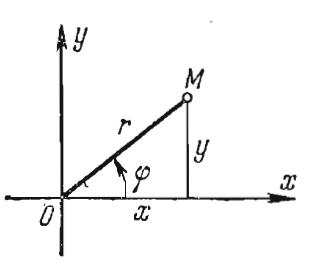
\includegraphics[width = 6cm]{polarCordinat}
$$
\iint_D f(x,y) dxdy = \iint_E f(r\cos \varphi, r\sin \varphi) r dr d\varphi
$$

\begin{title}[\Large]
  Использование цилиндрических координат при вычислении тройных интегралов
\end{title}

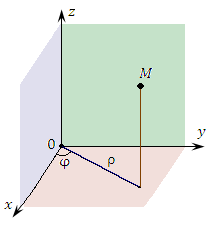
\includegraphics[width = 6cm]{cilindrCordinat}
$$
\left\{
\begin{array}{l}
  x = r \cos \varphi \\
  y = r \sin \varphi \\
  z = h
\end{array}
\right.
$$
$$
T  = \{ (r, \varphi, h): ~ r \ge 0 ~~ 0 \le \varphi < 2\pi ~~ h \in R \}
$$
$$
Y(r, \varphi, h) =
\left(
\begin{array}{ccc}
  \cos \varphi & -r \sin \varphi & 0 \\
  \sin \varphi & r \cos \varphi & 0 \\
  0 & 0 & 1
\end{array}
\right) = r
$$
$$
\iiint_E f(x, y, z) dxdydz = \iiint_D f(r\cos \varphi, r\sin \varphi, h) r
dr d\varphi dh
$$

\begin{title}[\Large]
  Использование сферических координат при вычислении тройных интегралов
\end{title}
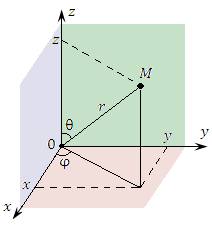
\includegraphics[width = 6cm]{spherCordinat}
$$
\left\{
\begin{array}{l}
  x = r \cos \psi \cos \varphi\\
  y = r \cos \psi \sin \varphi \\
  z = r \sin \psi
\end{array}
\right.
$$
$$
T = \left\{ (r, \varphi, \psi): ~ r \ge 0 ~~ \varphi \in [0, 2\pi] ~~ \psi \in
\left[-\frac{\pi}{2}, \frac{\pi}{2}\right] \right\}
$$
$$
Y(r, \psi, \varphi) =
\left(
\begin{array}{ccc}
  \cos \psi \cos \varphi &
  -r \cos \psi \sin \varphi &
  -r \sin \psi \cos \varphi \\

  \cos \psi \sin \varphi &
  r \cos \psi \cos \varphi &
  -r \sin \psi \sin \varphi \\

  \sin \psi & 0 & r \cos \psi
\end{array}
\right) = r^2 \cos \psi
$$
$$
\iiint_E f(x,y,z) dxdydz = \iint_D f(r\cos \psi \cos \varphi,
r\cos\psi \sin \varphi, r\sin \psi) r^2 \cos \psi dr d\varphi d\psi
$$

\begin{title}[\Large]
  Несобственные кратные интегралы
\end{title}

\begin{define}[исчерпания]
  $D \subset R^m ~ \{D_n\}$ называется исчерпание $D$ если

  1) открытые и измеримы по Жордану множества

  2) $\forall n \in N ~~ [D_n] \subset D_{n+1}$ (замыкание)

  3) $\cup_{n=1}^{\infty} D_n = D$
\end{define}

\begin{theorem}
  $\{D_n\} ~~ \{Q_n\}$ исчерпания $D \subset R^m$ тогда $\forall n \in N ~~
  \exists k_n \in N ~~ [D_n] \subset Q_{k_n}$
\end{theorem}

\begin{proof}
  От противного

  $\exists n_0 \in N ~~ \forall k \in N ~~ [D_{n_0}] \not\subset Q_k$
  $$
  \begin{array}{c}
    \exists x_1 \in [D_{n_0}] ~~ x_1 \not\in Q_1 \\
    \exists x_2 \in [D_{n_0}] ~~ x_2 \not\in Q_2 \\
    \cdots ~~~ \cdots ~~~ \cdots \\
    \exists x_n \in [D_{n_0}] ~~ x_n \not\in Q_n
  \end{array}
  $$
  $[D_{n_0}]$ замкнуто и ограничено так как измерено по Жордану

  Расмотрим последовательность $x_k$

  $\exists x_{n_k} \to a \in [D_{n_0}] \subset D_{n_0+1} \subset D ~~
  Q \in \cup_{k=1}^{\infty} Q_k$

  $\exists k_o \in N ~~ a \in Q_{k_0} ~~ \exists O_{\delta}(a) \subset Q_{k_0}$

  $x_{n_k} \to a ~~ \exists l \in N ~~ x_{n_k} \in O_{\delta}(a)$
\end{proof}

\begin{define}[несобственного кратного интеграла]
  $f(x) \ge 0$ непрерывна в $D \subset R^n$ тогда
  $$
  \lim_{n \to \infty} \int_{D_n} f(x) dx = \int_D f(x) dx
  $$
  если предел конечен то несобственный кратный интеграл сходится иначе
  расходится.
\end{define}

\begin{theorem}
  Определение несобственного интеграла коректно то есть не зависит от выбора
  исчерпаемого множества.
\end{theorem}

\begin{proof}
  $$
  \alpha_n = \int_{D_n} f(x) dx ~ \nearrow ~~ \beta_n = \int_{Q_n} f(x) dx ~
  \nearrow
  $$
  $$
  \alpha_n = \int_{D_n} f(x) dx \le \int_{Q_{k_n}} f(x) dx = \beta_{k_n} \le
  \lim_{n \to \infty} \beta_n = \beta
  $$
  $$
  \forall \alpha_n \le \beta ~~ \lim_{n \to \infty} \alpha_n = \alpha \le \beta
  $$
  $$
  \beta_n = \int_{Q_n} f(x) dx \le \int_{D_{k_n}} f(x) dx = \alpha_{k_n} \le
  \lim_{n \to \infty} \alpha_n = \alpha
  $$
  $$
  \forall \beta_n \le \alpha ~~ \lim_{n \to \infty} \beta_n = \beta \le \alpha
  $$
  $\Rightarrow ~ \alpha = \beta$
\end{proof}

\begin{theorem}
  Пусть $D \subset R^m$ возможно меняет знак
  $$
  f^+(x) = \frac{|f(x)| + f(x)}{2} ~~~
  f^-(x) = \frac{|f(x)| - f(x)}{2} ~~~
  f(x) = f^+(x) - f^-(x)
  $$
  $$
  \int_D f(x) dx = \int_D f^+(x) dx - \int_D f^-(x)dx
  $$
  сходится если оба интегрла сходятся иначе расходится.
\end{theorem}

\begin{title}[\Large]
  Приложения кратных интегралов
\end{title}
$$
\iint_D dx dy = S(D) ~ \text{площадь} ~ D
$$
$$
\iint_D \rho(x,y) dx dy = M(D) ~ \text{масса}
$$
$$
\iiint_T \rho(x,y,z) dx dy dz = M(T)
$$
$$
S_{oy} = \iint_D x \rho(x,y) dx dy ~~~ x_0 = \frac{S_{oy}}{M(D)}
$$
$$
I_{oy} = \iint_D x^2 \rho(x,y)dx dy ~~~ x_0 = \frac{I_{oy}}{M(D)}
$$